\documentclass[letterpaper,10pt]{article}

\usepackage{enumitem}
\usepackage{titling}
\usepackage{listings,listings-rust}
\usepackage{url}
\usepackage{soul}
\usepackage{hyperref}
\usepackage{setspace}
\usepackage{subfig}
\usepackage{sectsty}
\usepackage{pdfpages}
\usepackage{colortbl}
\usepackage{multirow}
\usepackage{multicol}
\usepackage{relsize}
\usepackage{amsmath}
\usepackage{wasysym}
\usepackage{fancyvrb}
\usepackage[yyyymmdd]{datetime}
\usepackage{amsmath,amssymb,amsthm,graphicx,xspace}
\usepackage[titlenotnumbered,noend,noline]{algorithm2e}
\usepackage[compact]{titlesec}
\usepackage{XCharter}
\usepackage[T1]{fontenc}
\usepackage[scaled]{beramono}
\usepackage[normalem]{ulem}
\usepackage{booktabs}
\usepackage{tikz}
\usetikzlibrary{arrows.meta,automata,shapes,trees,matrix,chains,scopes,positioning,calc,decorations.pathreplacing}
\tikzstyle{block} = [rectangle, draw, fill=blue!20, 
    text width=2.5em, text centered, rounded corners, minimum height=2em]
\tikzstyle{bw} = [rectangle, draw, fill=blue!20, 
    text width=4em, text centered, rounded corners, minimum height=2em]

\definecolor{namerow}{cmyk}{.40,.40,.40,.40}
\definecolor{namecol}{cmyk}{.40,.40,.40,.40}
\renewcommand{\dateseparator}{-}

\let\LaTeXtitle\title
\renewcommand{\title}[1]{\LaTeXtitle{\textsf{#1}}}

\lstset{basicstyle=\footnotesize\ttfamily,breaklines=true}

\newcommand{\CPP}{C\nolinebreak\hspace{-.05em}\raisebox{.4ex}{\tiny\bf +}\nolinebreak\hspace{-.10em}\raisebox{.4ex}{\tiny\bf +}}
\def\CPP{{C\nolinebreak[4]\hspace{-.05em}\raisebox{.4ex}{\tiny\bf ++}}}

\newcommand{\handout}[5]{
  \noindent
  \begin{center}
  \framebox{
    \vbox{
      \hbox to 5.78in { {\bf ECE459: Programming for Performance } \hfill #2 }
      \vspace{4mm}
      \hbox to 5.78in { {\Large \hfill #4  \hfill} }
      \vspace{2mm}
      \hbox to 5.78in { {\em #3 \hfill \today} }
    }
  }
  \end{center}
  \vspace*{4mm}
}

\newcommand{\lecture}[3]{\handout{#1}{#2}{#3}{Lecture#1}}
\newcommand{\tuple}[1]{\ensuremath{\left\langle #1 \right\rangle}\xspace}

\addtolength{\oddsidemargin}{-1.000in}
\addtolength{\evensidemargin}{-0.500in}
\addtolength{\textwidth}{2.0in}
\addtolength{\topmargin}{-1.000in}
\addtolength{\textheight}{1.75in}
\addtolength{\parskip}{\baselineskip}
\setlength{\parindent}{0in}
\renewcommand{\baselinestretch}{1.5}
\newcommand{\term}{Winter 2020}

\singlespace


\begin{document}

\lecture{5 --- Creating Processes \& Threads}{\term}{Patrick Lam and Jeff Zarnett}


\section*{Creating and Using Processes}


The workflow in UNIX is as follows. First, the parent spawns the child process with the \texttt{fork} system call. If it is interested in waiting for the child process to finish, it will use the system call \texttt{wait}, in which case the parent will be awaiting the completion of the child process. When the child process is finished, it returns a value with the \texttt{exit} system call. The parent process will then get this as the return value of the \texttt{wait} call and may proceed.

What does \texttt{fork} do? It creates a new process; it makes a copy of itself. The parent and child continue execution after the \texttt{fork} statement. If \texttt{fork} returns a negative number, the \texttt{fork} system call failed. If it returns 0, the process that got the 0 back is the child. If it returns a positive value, that is the process ID of the child.

After the \texttt{fork}, one of the processes may use the \texttt{exec} system call, or one of its variants, to replace its memory space with a new program. There's no rule that says this must happen; a child can continue to be a clone of its parent if it wishes. The \texttt{exec} invocation loads the binary file into memory and starts execution~\cite{osc}. At this point, the programs can go their separate ways, or the parent might want to wait for the child to finish. The parent is then blocked, waiting for the child process to execute.

Let's put this all together in an actual C-code example adapted from~\cite{osc}:

\begin{verbatim}
#include <sys/types.h>
#include <stdio.h> 
#include <unistd.h>

int main()
{
  pid_t pid;
  int childStatus;

  /* fork a child process */
  pid = fork();
  
  if (pid < 0) { 
  
    /* error occurred */ 
    fprintf(stderr, "Fork Failed"); 
    return 1;
    
 } else if (pid == 0) { 
    
    /* child process */
    execlp("/bin/ls","ls",NULL);
    
  } else { 
    
    /* parent process */
    /* parent will wait for the child to complete */
    wait(&childStatus);
    printf("Child Complete with status: %i \n", childStatus);
    
  }
    
  return 0;
}
\end{verbatim}

When executed, this code starts up and attempts to spawn a child process. Let us assume that the \texttt{fork} command succeeds and we do not enter the error-occurred block.  After the fork there are now two processes at the statement \texttt{ if ( pid < 0 ) } . The child process calls \texttt{execlp}, replacing itself with the \texttt{ls} (list directory contents) command. The parent process will go to the \texttt{wait} statement and wait for the child process to complete. The child process runs \texttt{ls}, listing the contents of the directory. Then it finishes. The parent process, finally, prints ``Child Complete'' to the console.

Thus, the output is:
\begin{verbatim}
jz@Freyja:~/fork$ ./fork 
fork   fork.c
Child Complete with status: 0
jz@Freyja:~/fork$ 
\end{verbatim}

Or, to represent this visually:

\begin{center}
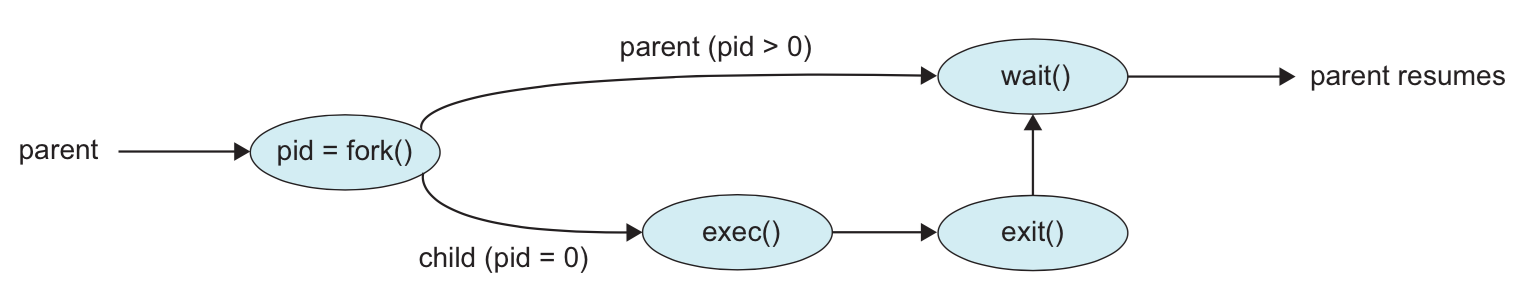
\includegraphics[width=0.85\textwidth]{images/fork-syscall.png}\\
Process creation with the \texttt{fork} system call~\cite{osc}.
\end{center}


\section*{Using Threads to Program for Performance}
We'll start by seeing how to use threads on ``embarrassingly parallel problems'':
  \begin{itemize}
    \item mostly-independent sub-problems (little synchronization); and
    \item strong locality (little communication).
  \end{itemize}

Later, we'll see:
  \begin{itemize}
    \item which problems are amenable to parallelization (\emph{dependencies})
    \item alternative parallelization patterns\\(right now, just use one thread
          per sub-problem)
  \end{itemize}

\paragraph{About Pthreads.} Pthreads stands for POSIX threads. It's available
on most systems, including Pthreads Win32 (which I don't recommend).
Use Linux, and our provided server, for this course. C++ 11 also includes threads
in its specification.

Here's a quick {\tt pthreads} refresher. To compile a C or C++ program
with pthreads, add the {\tt -pthread} parameter to the compiler
commandline. To ensure C++11 support in GCC, use \verb!-std=c++11!.

\paragraph{Starting a new thread.} You can start a thread with
\verb+pthread_create()+ or by creating a \verb+std::thread+:

{\small
  \begin{minipage}{.55\textwidth}
\begin{verbatim}
#include <pthread.h>
#include <stdio.h>

void* run(void*) {
  printf("In run\n");
}

int main() {
  pthread_t thread;
  pthread_create(&thread, NULL, &run, NULL);
  printf("In main\n");
}
\end{verbatim}
  \end{minipage} 
  \begin{minipage}{.4\textwidth}
\begin{verbatim}
#include <thread>
#include <iostream>

void run() {
  std::cout << "In run\n";
}

int main() {
  std::thread t1(run);
  std::cout << "In main\n";
  t1.join(); // see below
}
\end{verbatim}
  \end{minipage}
}

From the man page, here's how you use \verb+pthread_create+:
\begin{verbatim}
int pthread_create(pthread_t* thread, 
                   const pthread_attr_t* attr,
                   void* (*start_routine)(void*),
                   void* arg);
\end{verbatim}

\begin{itemize}
\item  {\bf thread}: creates a handle to a thread at pointer location

\item  {\bf attr}: thread attributes (NULL for defaults, more details later)

\item  {\bf start\_routine}: function to start execution

\item   {\bf arg}: value to pass to start\_routine
\end{itemize}

This function returns 0 on success and an error number otherwise (in
which case the contents of *thread are undefined).

\paragraph{Waiting for Threads to Finish.} If you want to join the threads
of execution, use the {\tt pthread\_join} call. Let's improve our example.

\begin{verbatim}
#include <pthread.h>
#include <stdio.h>

void* run(void*) {
  printf("In run\n");
}

int main() {
  pthread_t thread;
  pthread_create(&thread, NULL, &run, NULL);
  printf("In main\n");
  pthread_join(thread, NULL);
}
\end{verbatim}

The main thread now waits for the newly created thread to terminate
before it terminates. (C++11 requires threads to be either joined or
detached when they go out of scope; we'll see the meaning of detach below.)

Here's the syntax for {\tt pthread\_join}:

\begin{verbatim}
int pthread_join(pthread_t thread, void** retval)
\end{verbatim}
~\vspace*{-3em}
\begin{itemize}
\item  {\bf thread}: wait for this thread to terminate (thread must be~joinable).

\item  {\bf retval}: stores exit status of thread (set by {\tt pthread\_exit}) to
                 the location pointed by *retval. If cancelled, returns
                 {\tt PTHREAD\_CANCELED}. {\tt NULL} is ignored.
\end{itemize}

This function returns 0 on success, error number otherwise.

 {\bf Caveat: Only call this one time per thread!} Multiple calls to join on the same thread
  lead to undefined behaviour.

\paragraph{Inter-thread communication.} Recall that the {\tt pthread\_create} 
call allows you to pass data to the new thread. Let's see how we might do that\ldots

\begin{verbatim}
int i;
for (i = 0; i < 10; ++i)
  pthread_create(&thread[i], NULL, &run, (void*)&i);
\end{verbatim}

{\bf Wrong!} This is a \emph{terrible} idea. Why?
\begin{enumerate}
    \item The value of {\tt i} will probably change before the thread executes.
    \item The memory for {\tt i} may be out of scope, and therefore invalid by
          the time the thread executes.
\end{enumerate}
On the other hand, you can pull off something similar with C++11 threads:
\begin{verbatim}
int i;
for (i = 0; i < 10; ++i) {
  std::thread t(run, i);
  t.detach();
}
\end{verbatim}
This is OK because we pass {\tt i} by value, which doesn't work for Pthreads.

In Pthreads-land, this is marginally acceptable:
\begin{verbatim}
int i;
for (i = 0; i < 10; ++i)
  pthread_create(&thread[i], NULL, &run, (void*)i);

...

void* run(void* arg) {
  int id = (int)arg;
\end{verbatim}
It's not ideal, though.
  \begin{itemize}
    \item Beware size mismatches between arguments: you have
      no guarantee that a pointer is the same size as an int, so your data
      may overflow. (C only guarantees that the difference between two pointers is an int.)
    \item Sizes of data types change between systems. For maximum
      portability, just use pointers you got {\tt from malloc}.
  \end{itemize}

  The idiomatic way of returning data from threads in C++11 appears to be using
  futures. {\tt std::async} provides support for this:
\begin{verbatim}
#include <thread>
#include <iostream>
#include <future>

int run() {
  return 42;
}

int main() {
  std::future<int> t1_retval = std::async(std::launch::async, run);
  std::cout << t1_retval.get();
}
\end{verbatim}
This launches your thread for you. The {\tt get()} call waits until the answer
is ready and returns it to you.

\paragraph{More on inter-thread synchronization.} There was a comment on {\tt pthread\_join}
only working if the target thread was joinable. Joinable threads
(which is the default on Linux) wait for someone to call {\tt pthread\_join}
before they release their resources (e.g. thread stacks). On the other
hand, you can also create \emph{detached} threads, which release
resources when they terminate, without being joined. We've seen C++11 detached
threads above.

\begin{verbatim}
int pthread_detach(pthread_t thread);
\end{verbatim}
~\vspace*{-3em}
\begin{itemize}
\item  {\bf thread}: marks the thread as detached
\end{itemize}

This call returns 0 on success, error number otherwise.

Calling {\tt pthread\_detach} on an already detached thread results in undefined
behaviour.

\paragraph{Finishing a thread.} A thread finishes when its {\tt start\_routine}
returns. But it's also possible to explicitly end a thread from within:

\begin{verbatim}
void pthread_exit(void *retval);
\end{verbatim}
~\vspace*{-3em}
\begin{itemize}
\item  {\bf retval}: return value passed to function which called {\tt pthread\_join}
\end{itemize}

Alternately, returning from the thread's {\tt start\_routine} is equivalent
to calling {\tt pthread\_exit}, and {\tt start\_routine}'s return value
is passed back to the {\tt pthread\_join} caller. There is no C++11 equivalent.

\paragraph{Attributes.} Beyond being detached/joinable, threads have additional
attributes. (Note, also, that even though being joinable rather than
detached is the default on Linux, it's not necessarily the default everywhere).
Here's a list.
  \begin{itemize}
    \item Detached or joinable state
    \item Scheduling inheritance
    \item Scheduling policy
    \item Scheduling parameters
    \item Scheduling contention scope
    \item Stack size
    \item Stack address
    \item Stack guard (overflow) size
  \end{itemize}

Basically, you create and destroy attributes objects with {\tt
  pthread\_attr\_init} and {\tt pthread\_attr\_destroy}
respectively. You can pass attributes objects to {\tt
  pthread\_create}. For instance,

  \begin{verbatim}
size_t stacksize;
pthread_attr_t attributes;
pthread_attr_init(&attributes);
pthread_attr_getstacksize(&attributes, &stacksize);
printf("Stack size = %i\n", stacksize);
pthread_attr_destroy(&attributes);
  \end{verbatim}

Running this on a laptop produces:

  \begin{verbatim}
jon@riker examples master % ./stack_size 
Stack size = 8388608
  \end{verbatim}

Once you have a thread attribute object, you can set the thread state to joinable:
  \begin{verbatim}
pthread_attr_setdetachstate(&attributes,
                            PTHREAD_CREATE_JOINABLE);
  \end{verbatim}

\paragraph{Warning about detached threads.} Consider the following code.

\begin{verbatim}
#include <pthread.h>
#include <stdio.h>

void* run(void*) {
  printf("In run\n");
}

int main() {
  pthread_t thread;
  pthread_create(&thread, NULL, &run, NULL);
  pthread_detach(thread);
  printf("In main\n");
}
\end{verbatim}

  When I run it, it just prints ``In main''. Why?

\paragraph{Solution.} Use {\tt pthread\_exit} to quit if you have any detached threads.
  \begin{verbatim}
#include <pthread.h>
#include <stdio.h>

void* run(void*) {
  printf("In run\n");
}

int main() {
  pthread_t thread;
  pthread_create(&thread, NULL, &run, NULL);
  pthread_detach(thread);
  printf("In main\n");
  pthread_exit(NULL); // This waits for all detached
                      // threads to terminate
}
  \end{verbatim}
(There is no C++11 equivalent.)

%% \paragraph{Three useful Pthread calls.} You may find these helpful.

%% \begin{verbatim}
%% pthread_t pthread_self(void);

%% int pthread_equal(pthread_t t1, pthread_t t2);

%% int pthread_once(pthread_once_t* once_control,
%%                  void (*init_routine)(void));
%% pthread_once_t once_control = PTHREAD_ONCE_INIT;
%% \end{verbatim}

%% \begin{itemize}
%% \item {\tt pthread\_self} returns the handle of the currently running thread.
%% \item {\tt pthread\_equal} compares 2 threads for equality.
%% \item {\tt pthread\_once} runs a block of code just once, even across threads, based
%% on a (presumably-global) control variable. This is useful for initialization code.
%% \end{itemize}

\paragraph{Threading Challenges.}
  \begin{itemize}
    \item Be aware of scheduling (you can also set affinity with pthreads on
      Linux).

    \item Make sure the libraries you use are {\bf thread-safe}:
      \begin{itemize}
        \item Means that the library protects its shared data (we'll see how, below).
      \end{itemize}

    \item glibc reentrant functions are also safe: a program can have
      more than one thread calling these functions concurrently. For
      example, use {\tt rand\_r}, not {\tt
        rand}.
  \end{itemize}



\bibliographystyle{alphaurl}
\bibliography{459}


\end{document}
